\chapter{Dummy Variables}
\section{Dummy Variable}
\begin{align}
	P_i = \beta_0 + \beta_1 S_1 + \beta_2 D_i + \epsilon_i\\
	E(P_i) =
	\begin{cases}
		(\hat{\beta_0}+\hat{\beta_2})+\hat{\beta_1}S_i, &D_i = 1\\
		\hat{\beta_0} + \hat{\beta_1}S_i, &D_i = 0
	\end{cases}
\end{align}

\begin{figure}[htbp]
	\centering
	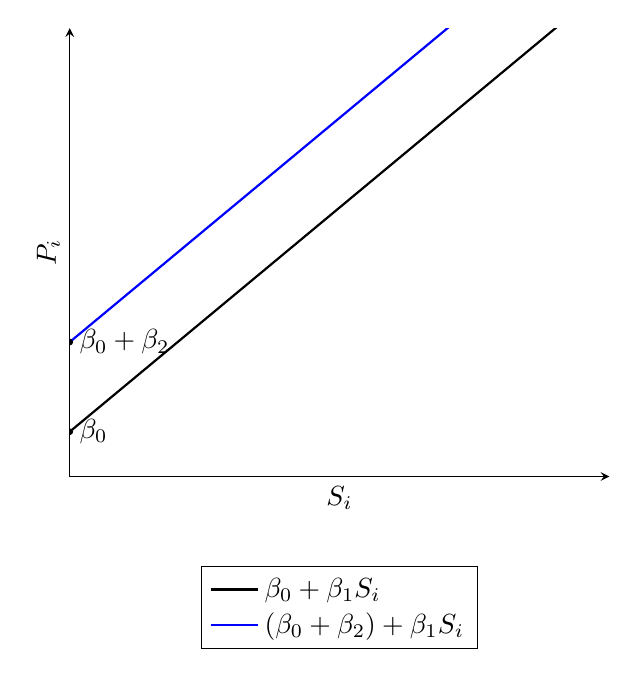
\begin{tikzpicture}
		\begin{axis}[axis lines = left, xmin = 0, ymin = 0, xmax = 10, ymax = 10, xlabel = $S_i$, ylabel = $P_i$, ticks=none, legend style={at={(0.5,-0.2)},anchor=north,legend cell align=left}]
			\addplot[domain=0:10,black, thick]{x+1};
			\addlegendentry{$\beta_0+\beta_1 S_i$}
			\addplot[domain=0:10,blue, thick]{x+3};
			\addlegendentry{$(\beta_0+\beta_2)+\beta_1 S_i$}
			\draw(axis cs:0,1)[fill]circle(1pt)node[right]{$\beta_0$};
			\draw(axis cs:0,3)[fill]circle(1pt)node[right]{$\beta_0+\beta_2$};
		\end{axis}
	\end{tikzpicture}
\end{figure}


\section{Slope Dummy Variable}
\begin{align}
	P_i = \beta_0 + \beta_1 S_1 + \beta_2 (S_i \cdot D_i) + \epsilon_i\\
	E(P_i) =
	\begin{cases}
		\hat{\beta_0} + \left(\hat{\beta_1}+\hat{\beta_2} \right)S_i, &D_i = 1\\
		\hat{\beta_0} + \hat{\beta_1}S_i, &D_i = 0
	\end{cases}
\end{align}

\begin{figure}[htbp]
	\centering
	\begin{tikzpicture}
		\begin{axis}[axis lines = left, xmin = 0, ymin = 0, xmax = 10, ymax = 10, xlabel = $S_i$, ylabel = $P_i$, ticks=none, legend style={at={(0.5,-0.2)},anchor=north,legend cell align=left}]
			\addplot[domain=0:10,black, thick]{0.5 * x+1};
			\addlegendentry{$\beta_0+\beta_1 S_i$}
			\addplot[domain=0:10,blue, thick]{x+1};
			\addlegendentry{$\beta_0+(\beta_1+\beta_2) S_i$}
			\draw(axis cs:0,1)[fill]circle(1pt)node[right]{$\beta_0$};
		\end{axis}
	\end{tikzpicture}
\end{figure}


\section{Slope \& Dummy Variable}
\begin{align}
	P_i = \beta_0 + \beta_1 S_1 + \beta_2  D_i + \beta_3 S_i D_i + \epsilon_i\\
	E(P_i) =
	\begin{cases}
		(\hat{\beta_0} + \hat{\beta_2}) + \left(\hat{\beta_1}+\hat{\beta_3} \right)S_i, &D_i = 1\\
		\hat{\beta_0} + \hat{\beta_1}S_i, &D_i = 0
	\end{cases}
\end{align}

\begin{figure}[htbp]
	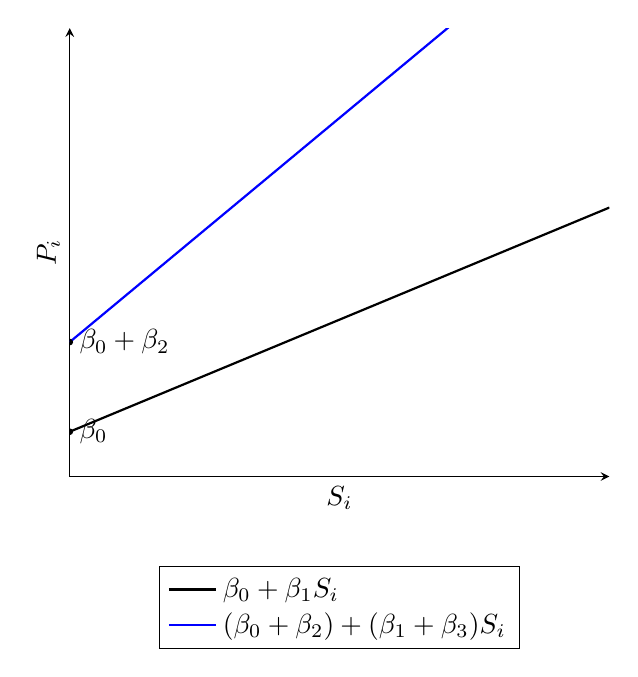
\begin{tikzpicture}
		\begin{axis}[axis lines = left, xmin = 0, ymin = 0, xmax = 10, ymax = 10, xlabel = $S_i$, ylabel = $P_i$, ticks=none, legend style={at={(0.5,-0.2)},anchor=north,legend cell align=left}]
			\addplot[domain=0:10,black, thick]{0.5 * x+1};
			\addlegendentry{$\beta_0+\beta_1 S_i$}
			\addplot[domain=0:10,blue, thick]{x+3};
			\addlegendentry{$(\beta_0+\beta_2)+(\beta_1+\beta_3) S_i$}
			\draw(axis cs:0,1)[fill]circle(1pt)node[right]{$\beta_0$};
			\draw(axis cs:0,3)[fill]circle(1pt)node[right]{$\beta_0+\beta_2$};
		\end{axis}
	\end{tikzpicture}
\end{figure}


\section{Multi-Categories Dummy Variable}
\begin{align}
	P_0 = b_0 \begin{pmatrix} 1 \\ 1 \\ 1\end{pmatrix} + \underbrace{b_1 \begin{pmatrix} 1 \\ 0 \\ 0\end{pmatrix} + b_2 \begin{pmatrix} 0 \\ 1 \\ 0\end{pmatrix} +b_3 \begin{pmatrix} 0 \\ 0 \\ 1\end{pmatrix}}_{\text{Leads to Perfect Multicollinearlity}}
\end{align}

\subsubsection{Alternatives}
\begin{itemize}
	\item $B_n$ captures the mean of each category, but F-Test is impossible\begin{align} y = \beta_1 D_{1i} + \beta_2 D_{2i} + \beta_3 D_{3i}\end{align}
	\item Computer drops automatically drops a variable \begin{align} y = \beta_0 + \beta_1 D_{1i} + \beta_2 D_{2i} + \beta_3 D_{3i} \end{align}
	\item Manually dropping a variable \begin{align} y = \beta_0 + \beta_1 D_{1i} + \beta_2 D_{2i} \end{align}
\end{itemize}
